\documentclass{tufte-handout}

\title{Resume}

\author{Matt Monihan. New York City}

%\date{28 March 2010} % without \date command, current date is supplied
\date{} % No Date
%\geometry{showframe} % display margins for debugging page layout

\usepackage{graphicx} % allow embedded images
  \setkeys{Gin}{width=\linewidth,totalheight=\textheight,keepaspectratio}
  \graphicspath{{graphics/}} % set of paths to search for images
\usepackage{amsmath}  % extended mathematics
\usepackage{booktabs} % book-quality tables
\usepackage{units}    % non-stacked fractions and better unit spacing
\usepackage{multicol} % multiple column layout facilities
\usepackage{lipsum}   % filler text
\usepackage{fancyvrb} % extended verbatim environments
  \fvset{fontsize=\normalsize}% default font size for fancy-verbatim environments
\usepackage[utf8]{inputenc}
\usepackage[english]{babel}
\usepackage{csquotes}

% Define colors
\definecolor{DarkGray}{RGB}{15,15,15}
\definecolor{LightGray}{RGB}{59,58,55}
\definecolor{BrightTaupe}{RGB}{252,246,219}
\definecolor{Taupe}{RGB}{191,186,166}
\definecolor{BurntOrange}{RGB}{198,100,13}
\definecolor{BrightRed}{RGB}{116,32,21}
\definecolor{SteelBlue}{RGB}{54,62,74}
\definecolor{LinkBlue}{RGB}{28,86,173}
\definecolor{HighlightBrown}{RGB}{46,110,87}

% Define Styles
\newcommand{\mhstandout}[1]{\textbf{\textcolor{DarkGray}{#1}}}
\newcommand{\shstandout}[1]{\textbf{\textcolor{BurntOrange}{#1}}}
\newcommand{\shyears}[1]{\small{\texttt{\textcolor{LightGray}{#1}}}}
\newcommand{\pstandout}[1]{\textcolor{BrightRed}{#1}}


% Define hyperlink info and PDF metadata
\hypersetup
{
    bookmarks=true,         % show bookmarks bar?
    unicode=false,          % non-Latin characters in Acrobat’s bookmarks
    pdftoolbar=true,        % show Acrobat’s toolbar?
    pdfmenubar=true,        % show Acrobat’s menu?
    pdffitwindow=false,     % window fit to page when opened
    pdfstartview={FitH},    % fits the width of the page to the window
    pdftitle={Curriculum Vitae - Matt Monihan},    % title
    pdfauthor={Matt Monihan},     % author
    pdfsubject={CV},   % subject of the document
    pdfcreator={Matt Monihan},   % creator of the document
    pdfproducer={MathBookAir}, % producer of the document
    pdfkeywords={cv} {resume} {experience}, % list of keywords
    pdfnewwindow=true,      % links in new window
    colorlinks=true,       % false: boxed links; true: colored links
    linkcolor=LinkBlue,          % color of internal links (change box color with linkbordercolor)
    citecolor=SteelBlue,        % color of links to bibliography
    filecolor=LinkBlue,      % color of file links
    urlcolor=LinkBlue           % color of external links
}


% Standardize command font styles and environments
\newcommand{\doccmd}[1]{\texttt{\textbackslash#1}}% command name -- adds backslash automatically
\newcommand{\docopt}[1]{\ensuremath{\langle}\textrm{\textit{#1}}\ensuremath{\rangle}}% optional command argument
\newcommand{\docarg}[1]{\textrm{\textit{#1}}}% (required) command argument
\newcommand{\docenv}[1]{\textsf{#1}}% environment name
\newcommand{\docpkg}[1]{\texttt{#1}}% package name
\newcommand{\doccls}[1]{\texttt{#1}}% document class name
\newcommand{\docclsopt}[1]{\texttt{#1}}% document class option name
\newenvironment{docspec}{\begin{quote}\noindent}{\end{quote}}% command specification environment

\begin{document}

\maketitle

\subsection{\textbf{Application Developer} at \shstandout{Miller Brothers Electrical Contracting} \shyears{[Apr 2015-Present]}}

\begin{marginfigure}%
  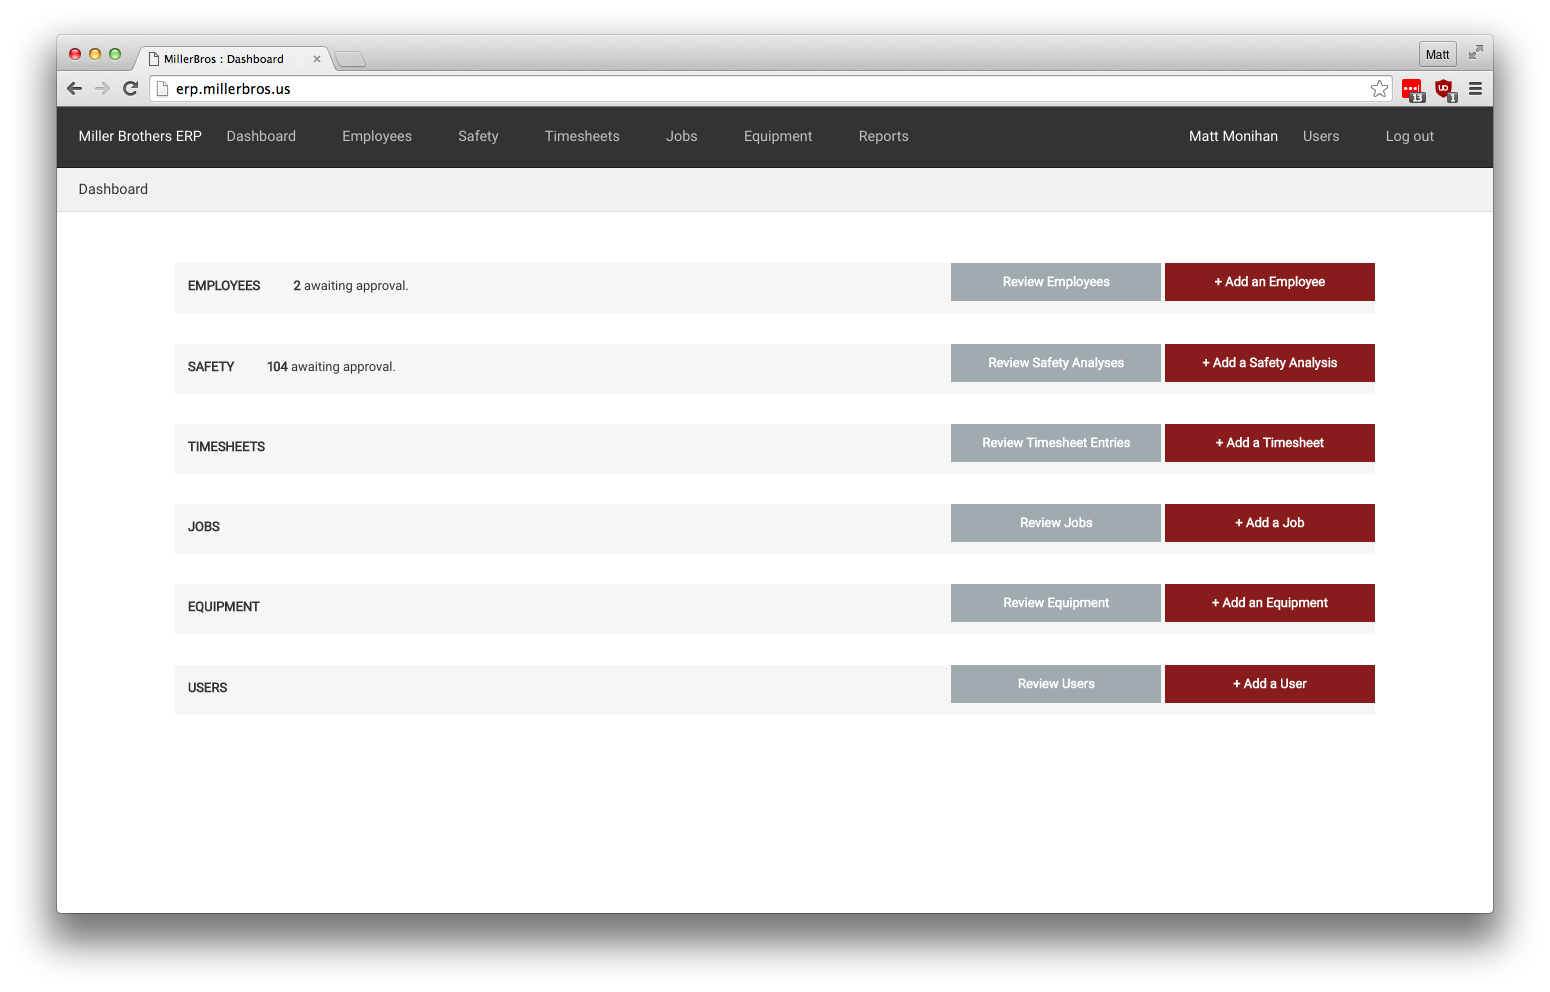
\includegraphics[width=\linewidth]{dashboard}
  \caption{Dashboard}
  \label{fig:dashboard}
\end{marginfigure}

\begin{marginfigure}%
  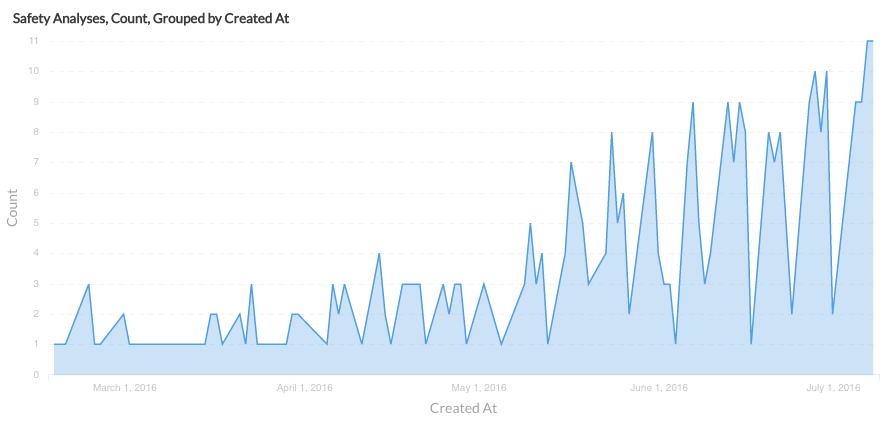
\includegraphics[width=\linewidth]{reports_by_day}
  \caption{Safety reports filed per day}
  \label{fig:reporting_dashboard}
\end{marginfigure}

Miller Brothers is a electrical contractor and solar installation provider in the Philadelphia and New Jersey region doing \$100M in sales annually. I was contracted to solve 3 key problems:

\begin{itemize}
\itemsep-0.1em
\item{On some work days, a union will send about 10 workers, some of which have never worked for the company. Collecting and verifying credentials, tax deductions and allocations is done on paper, and is an all-day process.}
\item{Every morning a foreman must complete a safety review. It is collected by the health and safety director where it is reviewed and stored in the event of an incident.}
\item{Finally, at the end of the day, a foreman must log the hours worked for each worker as well as the hours used for each piece of equipment. Each time sheet must be reviewed by an admin before being imported into a payroll system as well as Sage 300. There is no standardized format, so the admin has to wrangle entries coming in over the phone, via email, and on paper in various formats.}
\end{itemize}
\smallskip

\begin{figure}%
  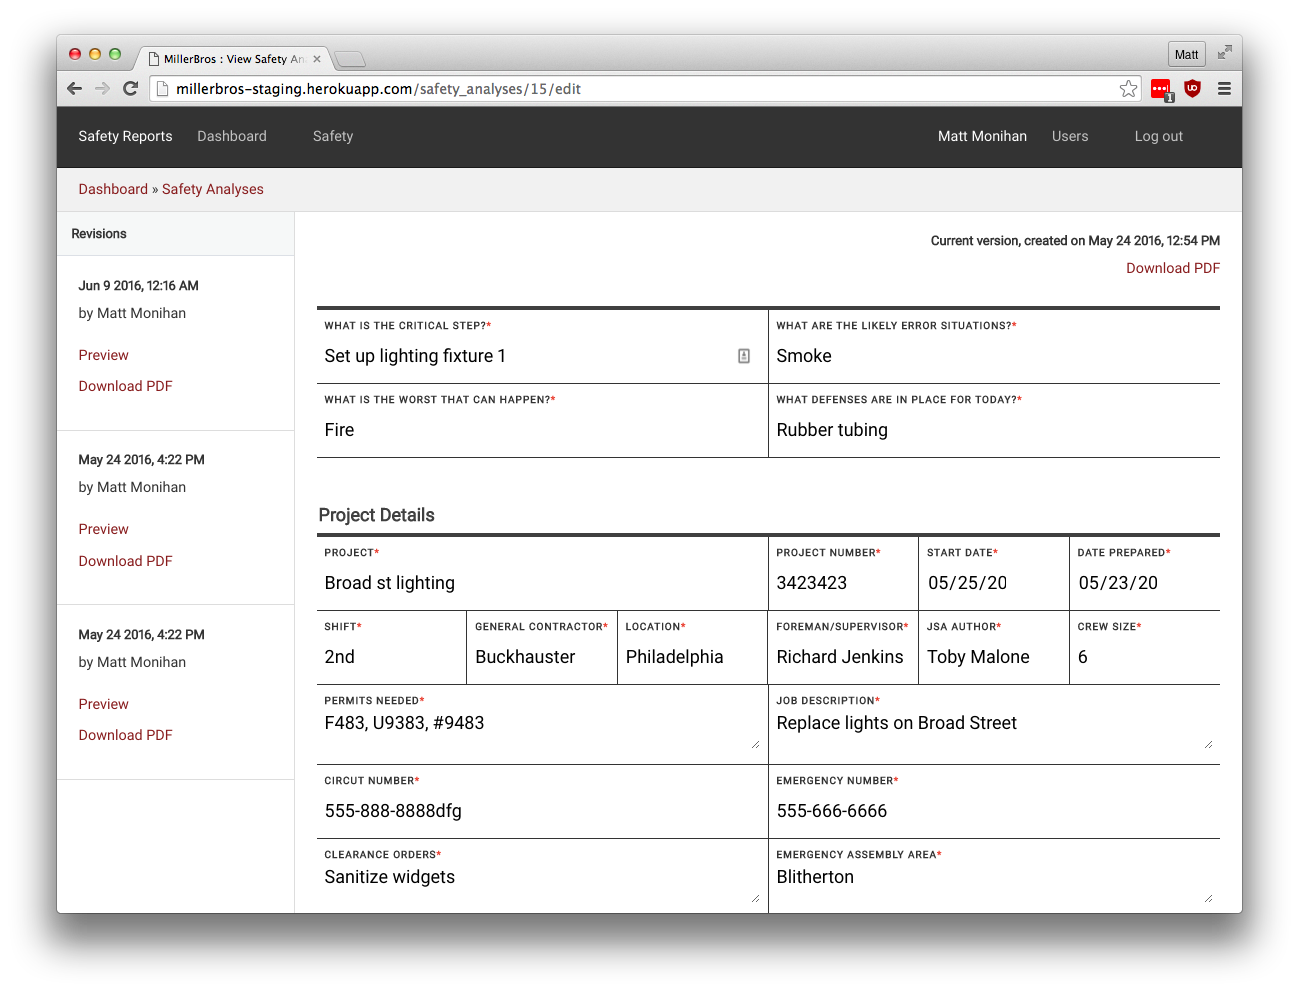
\includegraphics[width=\linewidth]{safety_report_item}
  \caption{Safety reporting interface showing multiple revisions and the ability to download as a PDF.}
  \label{fig:safety_report_item}
\end{figure}

I delivered a Ruby on Rails application that addresses each problem through the use of a mobile-first form, and a management interface. The application integrates with Docusign, Sage 300, and a payroll system called MPay.

The budget for the project was \$150k, was delivered 10\% early and has been in use for over 6 months. The company saves money by deploying new workers faster than ever, saving money on overnight shipping on paper forms, and eliminating errors due to inconsistent formats. This amounts to a savings of 45 minutes per foreman per day, which amounts to over \$60k in savings per year.




\subsection{\textbf{Product Manager} at \shstandout{RJMetrics, Inc.} \shyears{[Dec 2015-Present]}}

RJMetrics' vision is to inspire and empower data driven people. We do that by integrating with disparate data sources and consolidating it all into a data warehouse for analysis.

It's my job to conduct customer interviews, host and attend industry events, and build relationships that can produce valuable market intelligence for the product team.

In conjunction with my team, I provided the analysis and design inspiration for a new product, Pipeline, that was released to the market in November of 2015.

It is a pleasure to work with this team, and be surrounded by some of the smartest minds of our time.

\subsection{\textbf{Lead UX Designer} at \shstandout{RJMetrics, Inc.} \shyears{[Nov 2011-Dec 2015]}}

I joined the team as the 10th employee and led initiatives to improve the user experience.

I managed a team of developers that is solving one of the most challenging UX problems of our time: how to make sense of data. With over 1,800+ potential marketing technology data sources, our system needed to be robust to handle the different types of data sent through our pipeline, and the interface needed to be exceptionally flexible.

One of my biggest projects, the report builder, entailed a team of 5 to design, architect, and execute a complete overhaul of our chart building work flow. The project took 6 months, and was measured by the time it took for both experts and novices to complete a battery of test analyses.

We set up both formal and informal user tests throughout the development process that showed vast improvement in the time to create an analysis. In most cases, we saw improvements of about 50\% with certain use cases with 100\%+ improvements.

\begin{figure}%
  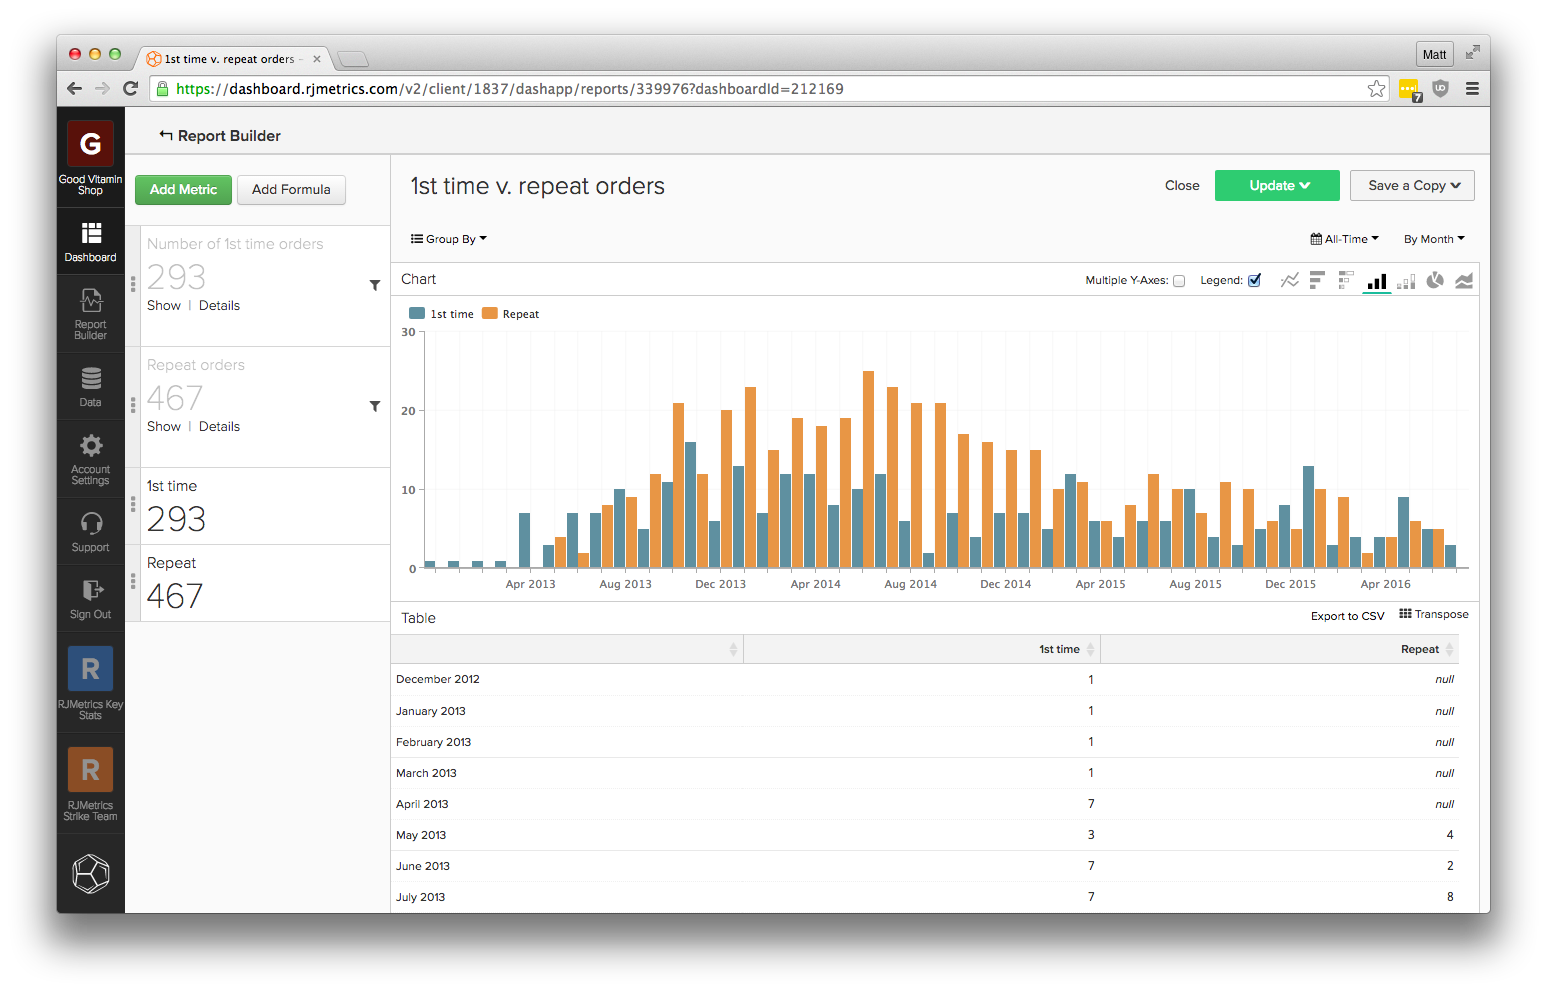
\includegraphics[width=\linewidth]{report_builder}
  \caption{The final report builder interface showing multiple metrics (1st time and repeat orders) being calculated and display with both instantaneous aggregate values(on the left) and those values over time.}
  \label{fig:report_builder}
\end{figure}

\pagebreak

Most remarkable were the analyses that could now be created that had been just too time consuming to be produced with the previous system. In real terms, this meant an analysis that took 1 hour to complete(begrudgingly) could be completed in under 5 minutes.

Our customers, and analysts had this to say:

``This will save me hours of time, it already has.``
An RJMetrics Analyst.

``Using the Report Builder is like Christmas.``
An RJMetrics Customer.

``As soon as prospects open our chart editor, their likelihood of converting into paying customers skyrockets.``
Robert Moore, CEO, RJMetrics as quoted in the NYTimes

\subsection{\textbf{Cofounder, Director of User Experience (UX)} at \shstandout{Jarvus Innovations} \shyears{[Jan 2011-Oct 2011]}}

My role at Jarvus was to manage the experience for our clients'​ users. My responsibilities ranged from project management to diving in and writing code. I designed information architecture artifacts including wire frames, use cases, and activity diagrams, and then ensured that they were implemented in a way that maintained a high-quality user experience.
While at Jarvus I led the execution of both the Consumer Reports Mobile Shopper 2011, and the Christie's Auction Mobile Application using the cutting edge Sencha Touch Framework.

\section{\mhstandout{Projects}}
\begin{itemize}
\itemsep-0.1em
\item{Consumer Reports Mobile Shopper 2011}
\item{Christies iPhone Application}
\item{GetDynamicWear.com}
\item{CreditScoutApp.com}
\item{PhillyTechWeek.com}
\item{TEDxPhilly.com (2010)}
\item{TEDxSJU (2011)}
\item{TheRoots.com}
\item{AppsForSepta.org}
\end{itemize}
\smallskip

\subsection{\textbf{Web Development Evangelist} at \shstandout{Devnuts} \shyears{[Dec 2009-Oct 2011]}}

My job at Devnuts was to listen to the members of our community and provide guidance related to software development and business planning. I've advised over 50 startups and entrepreneurs in Philadelphia.

My role also included managing the office with my partners and hosting events including the SEPTA Hackathon on October 8th 2011(http://appsforsepta.org/).

http://www.devnuts.com/


\subsection{\textbf{Undergrad} at \shstandout{Drexel University} \shyears{[Sep 2005-Jun 2010]}}
I completed Drexel's 5-year program in Business Administration including 3 6-month full-time internships. The first, as a portfolio manager at Valley Forge Asset Management. The second, as a web developer at FullSix. And, the third, as a web developer for a medical news website built for a team of investors.


\end{document}
